
\subsubsection{Integration of Strain Gauge}

\indent Figure \ref{fig:OmegaSoldered} is one of the 3-element rosette strain gauges with pre-soldered ribbon leads. Purchased from omega engineering with
model number SGD-6/120RYT23. These strain gauges were necessary after realizing the difficulty of soldering leads to the original set of strain gauges.
The pre-soldered ribbon leads on the second set of strain gauges also proved to be unsuccessful during experimentation. This was because the leads would
not stay secured to the attaching clips while tests were being run. Even with the persistent attempts to get the strain gauges connected and working
correctly, the data received was still very inaccurate. One possible contributing factor to this may have be the lack of precision when applying the
strain gauge to the exact location on the beam. However, one definite factor that contributed to the inaccurate data from the strain gauges was the
type of strain gauge that was used. A strain gauge with a different gauge factor and a higher resistance would have been more favorable. The higher
the resistance of a strain gauge, the higher the sensitivity. The original sets of strain gauges had a resistance of 120 $\Omega$, but to precisely
measure strain on a beam the resistance must be much higher, 350 $\Omega$ or more. The costs for a pack of 6 similar strain gauges with a
resistance of 350 $\Omega$ from omega engineering is one hundred dollars. Another factor that haulted the efforts to apply the strain gauge was
that they required another ADC output. It is possible to make more outputs, however this also demands that the time synchronization is even more
accurate. Nevertheless, higher resistant strain gauges would be better for sensor packages for future developments. \\

\begin{figure}[h!]
\centering
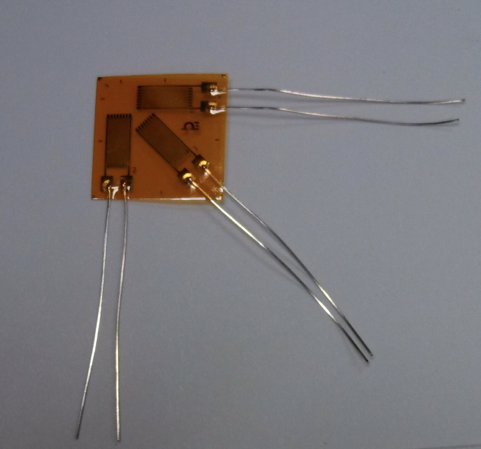
\includegraphics[width=\textwidth]{./MCINTOSH_Images/Strain_Gauge_with_Leads.png}
\caption{Omega 3-Element Rosette with pre-soldered leads.}
\label{fig:OmegaSoldered}
\end{figure}

\subsubsection{Package Assembly}

\paragraph{Package Location}
\indent Figure \ref{fig:PackageLocation} is an abaqus visualization of the Newport Bridge with the proposed location for the sensor package to be mounted.
As shown in the figure, the center of the bridge is the best location for the sensor package. This is because the greatest amplitude of displacement will
occur during the first mode of vibration at the middle of the bridge. Mounting the sensor package to the bridge must be done without damaging the
structure in any way. The sensor package must also be capable of being moved easily. Most importantly, the package must be secured without any of its
own motion, this is so that the sensors can recognize the movement of the bridge and not the package itself. The most economical way of securing the
sensor package to the bridge is to use powerful magnets. Neodymium Magnets are strong magnets that work well in all environments and resist
demagnetization. One negative aspect of the magnets is that it can be prone to corrosion if not protected with a coating properly. There is also a
concern that the magnetic field can disrupt the electronics within the case. However, these issues can be prevented if the correct precautions are
taken. The magnets come in many shapes and sizes, shown in Figure \ref{fig:PackageLocation} one can see that the magnets can be bought with pre
made holes for screws for mounting to the package. The magnets in figure \ref{fig:PackageLocation} are model MMR-A-XC from KJMagnetics.com. This
magnet is hardly larger than a penny, yet it can easily be screwed into the sensor package and pull a force of 54.14 pounds. With two of these
magnets screwed into the sensor package the package would be secured to the bridge. If calculations are run to prove the wind speed on the
surface of the package to be too much for this pull force, stronger magnets are available. KJMagnetics.com also has similar magnets but with
different pull forces ranging from 26.8 pounds to 260 pounds. These magnets can be used for securing the solar panels and wind turbine as
well. Figure \ref{fig:Proposed Package, Panels and Turbine Location} shows a practicable location for the sensor package along with the solar
panels above and the wind turbine hanging just below. The sensor package should be mounted on the outside of one of the major vertical beams
at midspan of the bridge. The solar panels and wind turbine must be mounted close within a reasonable distance to keep the cable length to
a minimum. The best place to mount the solar panels is on top of the upper horizontal beam on the southern side of the bridge. This will
allow for the most amount of sun light and the shortest amount of cable necessary. The best place to mount the wind turbine is on the
bottom of the lower horizontal beam on the southern side of the bridge. This location has plenty of wind because it is above the middle
of the Narragansett Bay. By mounting the sensor package, solar panels and wind turbine below the deck on the southern side of the
bridge the package will be capable of producing its own power and accurately measuring the vibrations of the bridge.


\begin{figure}[h]
\centering
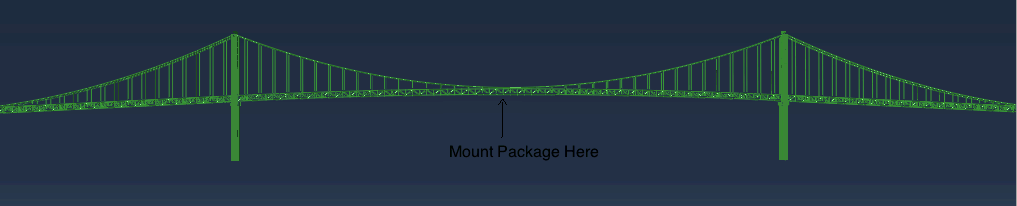
\includegraphics[width=\textwidth]{./MCINTOSH_Images/Bridge_Full_.png}
\caption{Proposed Package Mounting Location.}
\label{fig:PackageLocation}
\end{figure}

\begin{figure}[h]
\centering
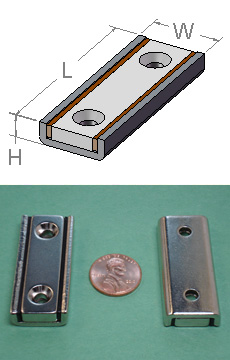
\includegraphics[width=\textwidth]{./MCINTOSH_Images/Neodymium_Mounting_Magnet.jpg}
\caption{Neodymium Mounting Magnet.}
\label{fig:Mounting Magnet}
\end{figure}

\begin{figure}[h]
\centering
\includegraphics[width=\textwidth]{./MCINTOSH_Images/Proposed_Package_Location.png}
\caption{Proposed Location for Sensor Package, Wind Turbine and Solar Panels.}
\label{fig:Proposed Package, Panels and Turbine Location}
\end{figure}

